\documentclass{beamer}
\usetheme{Madrid}
\usecolortheme{default}

\usepackage{amsmath}
\usepackage{amssymb}
\usepackage{graphicx}
\usepackage{booktabs}
\usepackage{xcolor}

\title[Option Skew Statistical Arbitrage]{Statistical Arbitrage via\\Option Volatility Skew}
\subtitle{MS\&E 244 Project}
\author{Sondre Rogde \and Bjorn Thor}
\date{\today}

\begin{document}

%--- Title Slide ---
\begin{frame}
  \titlepage
\end{frame}

%--- Table of Contents ---
\begin{frame}{Outline}
  \tableofcontents
\end{frame}

%=============================================================
\section{Strategy Overview}
%=============================================================

\begin{frame}{Strategy Overview}
  \begin{block}{Core Idea}
    Use option-implied volatility skew as a cointegrated signal between
    individual stocks and their sector ETFs.
  \end{block}
  \vspace{0.5em}
  \begin{enumerate}
    \item Compute the \textbf{volatility surface} from option data for each ticker
    \item Extract the \textbf{implied volatility skew} as a scalar time series
    \item Model the \textbf{cointegration} between stock skew and sector ETF skew
    \item Trade the \textbf{mean-reverting spread} between the two
    \item \textbf{Delta-hedge} to remove exposure to the underlying equity
  \end{enumerate}
\end{frame}

%=============================================================
\section{Data \& Cleaning}
%=============================================================

\begin{frame}{Data \& Cleaning}
  \begin{columns}
    \column{0.5\textwidth}
      \textbf{Raw Data}
      \begin{itemize}
        \item $\sim$10 GB of option data
        \item Sample period: \textbf{2015--2019}
      \end{itemize}
      \vspace{0.8em}
      \textbf{Filters Applied}
      \begin{itemize}
        \item Remove options with $< 1$ week to expiration\\
              {\small (noisy near expiry)}
        \item Remove options with implied volatility $> $ threshold\\
              {\small (some values exceeded 800\%)}
      \end{itemize}
    \column{0.5\textwidth}
      \begin{exampleblock}{Why These Filters?}
        Very short-dated options exhibit large bid-ask spreads and
        gamma blow-ups that distort the skew estimate.
        Extreme IV values are data errors or illiquid deep-OTM strikes.
      \end{exampleblock}
  \end{columns}
\end{frame}

%=============================================================
\section{Methodology}
%=============================================================

\begin{frame}{Step 1 --- Constructing the Skew}
  \textbf{For each day and each ticker:}
  \vspace{0.5em}
  \begin{enumerate}
    \item Fix a target time-to-expiration $\tau^*$
    \begin{itemize}
      \item If $\tau^*$ is unavailable, linearly interpolate from the two
            nearest available maturities
    \end{itemize}
    \item Use \textbf{OTM calls and OTM puts only}
    \begin{itemize}
      \item Higher liquidity; avoids early-exercise noise
      \item Future extension: weight by open interest
    \end{itemize}
    \item Fit a \textbf{second-degree polynomial} to the implied volatility smile
          as a function of log-moneyness $\kappa = \log(K/S)$:
    \[
      \sigma_{IV}(\kappa) \approx \beta_0 + \beta_1 \kappa + \beta_2 \kappa^2
    \]
    \item Interpret $\hat{\beta}_1$ as the \textbf{skew}
  \end{enumerate}
  \vspace{0.3em}
  \begin{alertblock}{Alternative}
    More advanced techniques (e.g.\ signature methods, SVI parametrisation)
    could capture higher-order surface geometry.
  \end{alertblock}
\end{frame}

\begin{frame}{Step 2 --- Trading the Spread}
  We now have skew time series $\{s_t^{\text{stock}}\}$ and
  $\{s_t^{\text{sector}}\}$.
  \vspace{0.5em}
  \begin{enumerate}
    \item \textbf{Cointegration regression}
    \[
      s_t^{\text{stock}} = \alpha + \beta \, s_t^{\text{sector}} + \varepsilon_t
    \]
    \item \textbf{Rolling z-score} of residuals $\varepsilon_t$
    \[
      z_t = \frac{\varepsilon_t - \mu_{\varepsilon}}{\sigma_{\varepsilon}}
    \]
    \item \textbf{Entry / exit rules} (mean-reversion):
    \begin{itemize}
      \item Enter when $|z_t| > z_{\text{entry}}$
      \item Exit when $|z_t| < z_{\text{exit}}$
    \end{itemize}
    \item \textbf{Position sizing}: if spread is high, go long stock-skew
          reversion and short sector-skew reversion, weighted by $\hat\beta$
  \end{enumerate}
\end{frame}

\begin{frame}{Step 3 --- Delta Hedging}
  \begin{block}{Why Delta Hedge?}
    A pure options spread position carries first-order equity exposure.
    We neutralise this to isolate the \emph{skew} signal.
  \end{block}
  \vspace{0.5em}
  \begin{itemize}
    \item Compute Black-Scholes $\Delta$ for each option leg
    \item Trade the underlying stock / ETF to flatten the net delta daily
    \item This converts the strategy into a \textbf{volatility / skew trade},
          independent of equity market direction
  \end{itemize}
  \vspace{0.5em}
  \begin{exampleblock}{Hysteresis Band}
    Entry threshold $z_{\text{entry}}$ and exit threshold $z_{\text{exit}}$
    are tuned to reduce transaction costs from excessive rebalancing.
  \end{exampleblock}
\end{frame}

%=============================================================
\section{Results}
%=============================================================

\begin{frame}{Cumulative Returns}
  \begin{center}
    % Replace with: 
\includegraphics[width=0.85\textwidth]{../plots/option_skew/cumulative_returns.png}
    \vspace{2cm}
    \textbf{[PLACEHOLDER --- cumulative returns chart]}
    \vspace{2cm}
  \end{center}
\end{frame}

\begin{frame}{Annual Returns}
  \begin{center}
    % Replace with: 
\includegraphics[width=0.85\textwidth]{../plots/option_skew/annual_returns.png}
    \vspace{2cm}
    \textbf{[PLACEHOLDER --- annual returns bar chart]}
    \vspace{2cm}
  \end{center}
\end{frame}

\begin{frame}{Drawdown}
  \begin{center}
    % Replace with: 
\includegraphics[width=0.85\textwidth]{../plots/option_skew/drawdown.png}
    \vspace{2cm}
    \textbf{[PLACEHOLDER --- drawdown chart]}
    \vspace{2cm}
  \end{center}
\end{frame}

\begin{frame}{P\&L Decomposition}
  \begin{center}
    % Replace with: 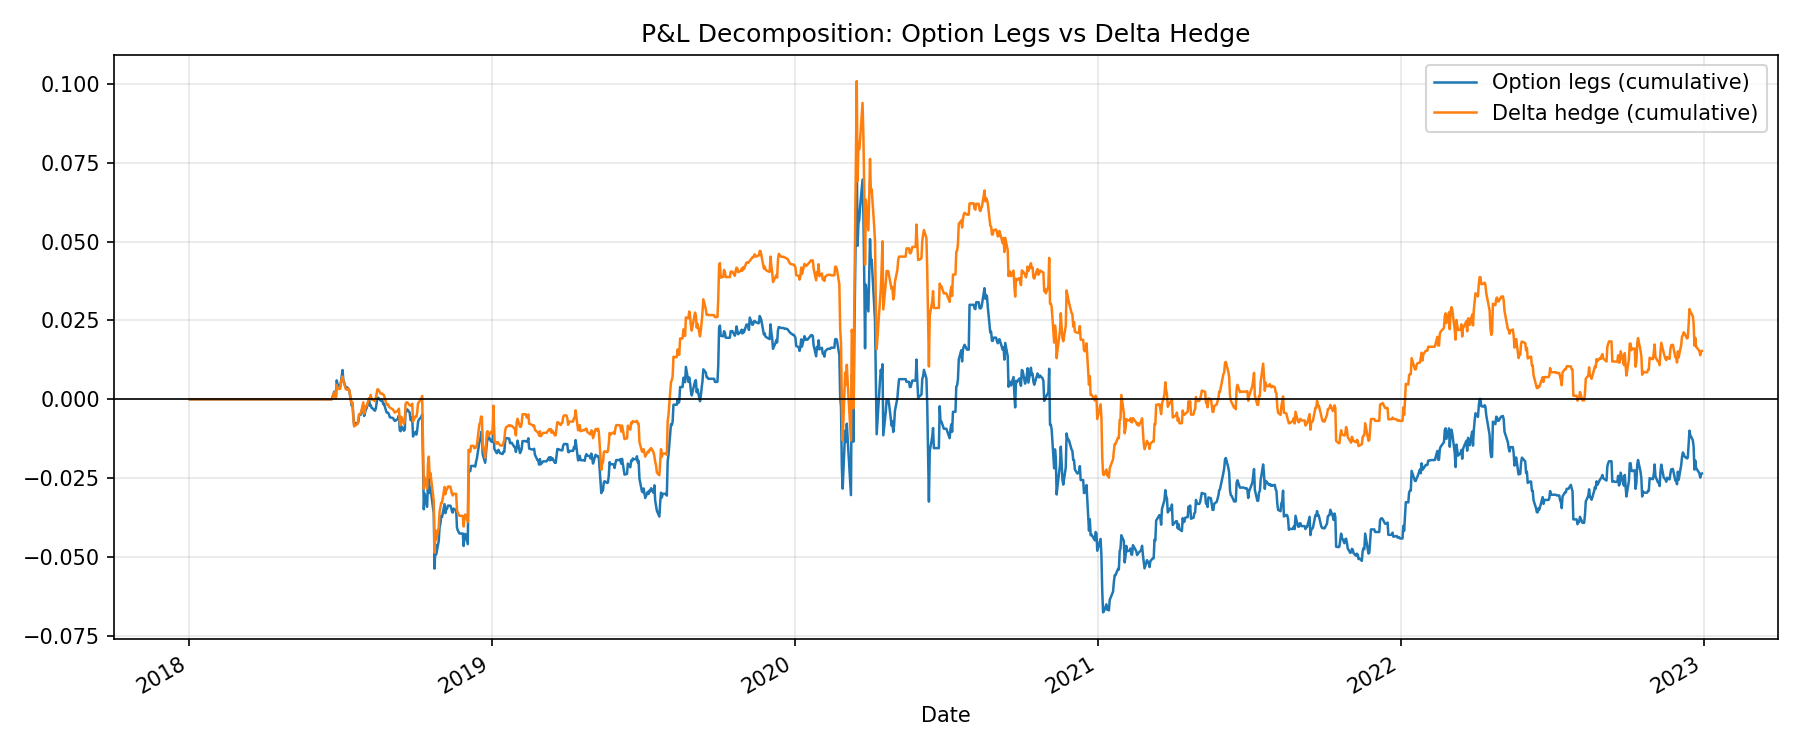
\includegraphics[width=0.85\textwidth]{../plots/option_skew/pnl_decomposition.png}
    \vspace{2cm}
    \textbf{[PLACEHOLDER --- P\&L decomposition]}
    \vspace{2cm}
  \end{center}
\end{frame}

\begin{frame}{Signals}
  \begin{center}
    % Replace with: 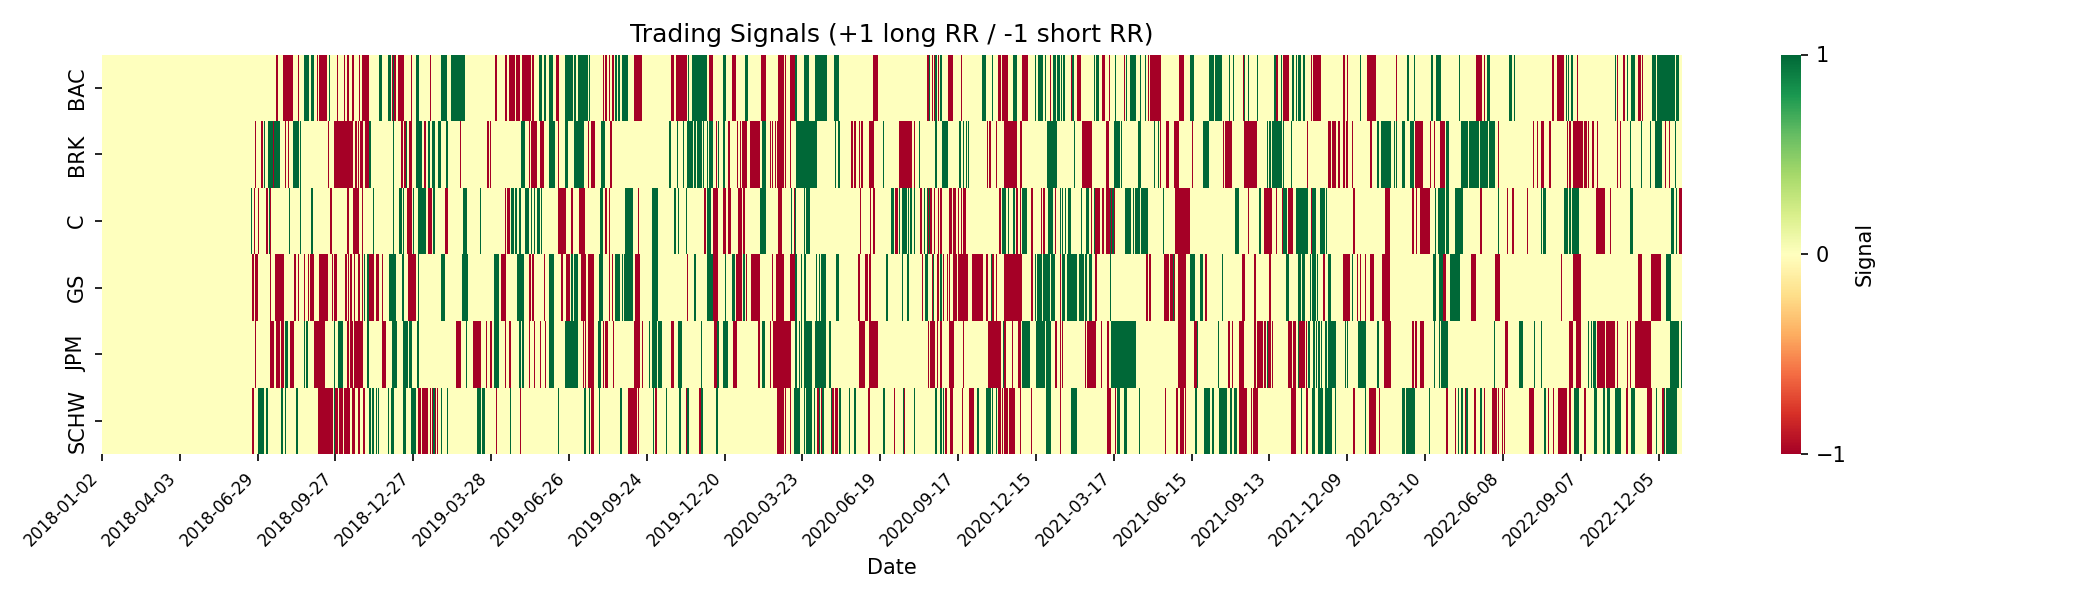
\includegraphics[width=0.85\textwidth]{../plots/option_skew/signals.png}
    \vspace{2cm}
    \textbf{[PLACEHOLDER --- entry/exit signal chart]}
    \vspace{2cm}
  \end{center}
\end{frame}

\begin{frame}{Monthly Returns Heatmap}
  \begin{center}
    % Replace with: 
\includegraphics[width=0.85\textwidth]{../plots/option_skew/monthly_returns.png}
    \vspace{2cm}
    \textbf{[PLACEHOLDER --- monthly returns heatmap]}
    \vspace{2cm}
  \end{center}
\end{frame}

%=============================================================
\section{Conclusion}
%=============================================================

\begin{frame}{Conclusion \& Future Work}
  \begin{columns}
    \column{0.5\textwidth}
      \textbf{Summary}
      \begin{itemize}
        \item Extracted skew from option surface via polynomial fit
        \item Traded cointegrated stock--sector skew spread
        \item Delta-hedged to isolate skew signal
      \end{itemize}
    \column{0.5\textwidth}
      \textbf{Future Extensions}
      \begin{itemize}
        \item Use full volatility surface (not just one $\tau$)
        \item Weight by open interest
        \item SVI / signature-method skew parametrisation
        \item Richer cointegration models (Engle-Granger, Johansen)
        \item Transaction cost modelling
      \end{itemize}
  \end{columns}
  \vspace{1em}
  \begin{block}{Key Takeaway}
    Option skew cointegration provides a market-neutral, delta-hedged
    signal with meaningful mean-reversion properties.
  \end{block}
\end{frame}

\begin{frame}
  \centering
  \Large Thank you!\\[1em]
  \normalsize Questions?
\end{frame}

\end{document}
